\documentclass{article}
\usepackage[utf8]{inputenc}
\usepackage[spanish]{babel}
\usepackage{graphicx, graphics, float}
\usepackage[a4paper, total={6in, 10in}]{geometry}
\title{DSD Memoria Práctica 3}
\author{Andrés Merlo Trujillo}
\date{}
\begin{document}
%TODO: MUY IMPORTANTE COMPROBAR LOS DE LAS INSTANCIAS DEL SERVIDOR, SEGURAMENTE ESTE MALY SE REFIERA A INSTANCIAS DEL METODO REMOTO O ALGO
%TODO 2: PLANTEAR EN ELIMINAR EL APARTADO DE IMPLEMENTACION YA QUE APARECE EN EL PDF
%TODO 3: QUIZAS PONER LOS METODOS QUE SE MENCIONAN EN LA PARTE 2 COMO UNA LISTA
%TODO 4: EXPLICAR UN POCO MAS LA PALABRA CLAVE SYNCHRONIZED
%TODO 5: EXPLICAR EL USO DE LAS VARIABLES VOLATILES
\maketitle

\section{Estructura de carpetas y explicación de distintos scripts}
Esta sección solo sirve a modo de explicación de como estan estructuradas las carpetas de esta practica. En el directorio raiz se encuentran 4 carpetas, 3 de ellas correspondientes a los ejemplos y la ultima, denominada ``Parte 2'', destinada al ejercicio del servidor de donaciones.

Dentro de la carpeta ``Parte 2'' se encuentran dos que explicaré a continuación:

%PONER LA ESTRUCTURA EN CARPETAS
%HACER UNA LISTA CON SUBLISTAS CUANDO YA SE TENGA UNA ESTRUCTURA FINAL


De manera general, para ejecutar todos los ejemplos, incluido el servidor de donaciones, es necesario siempre lanzar el script ``script\_server.sh'' y luego lanzar alguna de las variaciones del ``script\_cliente.sh''.



\section{Primera parte, Ejemplos}
En esta primera parte se pide copiar los códigos de prueba que aparecen en el guión de prácticas y comentar como funcionan y qué hacen.

\bigskip

Lo primero que hay que hacer es tener instalado una versión de OpenJDK lo suficientemente antigua porque si no al usar el comando \textit{javac *.java} saldrá un error similar a este:

%INSERTAR ERROR DE COMPILACIÓN

En mi caso tenía la versión 18 de JDK y he tenido que descargarme la versión 11 de la misma y configurarla para que sea la que se use por defecto.

\bigskip

Algo interesante que me ha ocurrido (no sé si ha sido mucha casualidad, pero he probado la ejecución varias veces) es que estaba usando la versión de JDK 8 y en la primera parte del ejemplo 2 se daba bien la ejecución de las hebras sin haber entrelazamientos y sin usar la palabra clave \textit{synchronized}. Como me extrañaba, probé la última versión que tenía disponible mi distribución antes de dar error de compilación, que en este caso es la versión 11, como he dicho anteriormente. Con la versión 11 si se producen entrelazamientos, por lo que supongo que es problema de la versión.

\bigskip
%QUIZAS HAGA FALTA ELIMINAR ESTO
Otro problema que he tenido esa la hora de usar el script, ya que dentro del mismo se lanzan secuencialmente el servidor y los clientes, esto produce que se lancen nada más que el servidor y que los clientes no se lancen.

%FOTO DE LO OCURRIDO
Para ello he separado la parte de la invocación de los clientes en otro script para poder lanzar ambos en dos terminales distintas.

\subsection{Ejemplo 1}
\subsubsection{Descripción}
Este ejemplo lo que realiza en el lado del cliente es llamar al método remoto \textit{escribir\_mensaje} con el identificador pasado por consola del cliente.

En el lado del servidor al ejecutar el método hay dos opciones, si el identificador pasado acaba en 0 entonces duerme durante 5000 ms (5 segundos), en otro caso simplemente indica que ha recibido la petición y muestra el identificador del cliente.

%FOTO CON ALGUNA EJECUCION
\begin{figure}[H]
    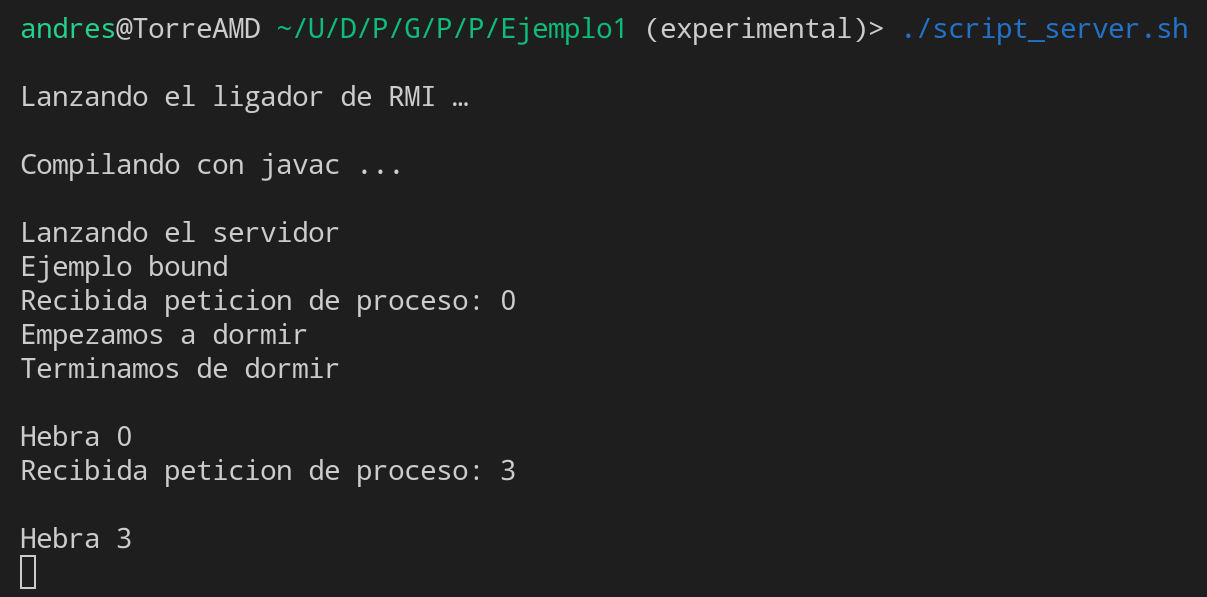
\includegraphics[width=\textwidth]{imagenes/E1S.png}
    \caption{Salida del servidor al ejecutar los clientes}
\end{figure}

Como se puede observar el primer cliente que se lanza tiene el identificador 0, por lo que se pone a dormir y se indica en el servidor. El siguiente, que tiene identificador 3, simplemente hace que se muestre en el servidor su información, pero no se duerme.

\begin{figure}[H]
    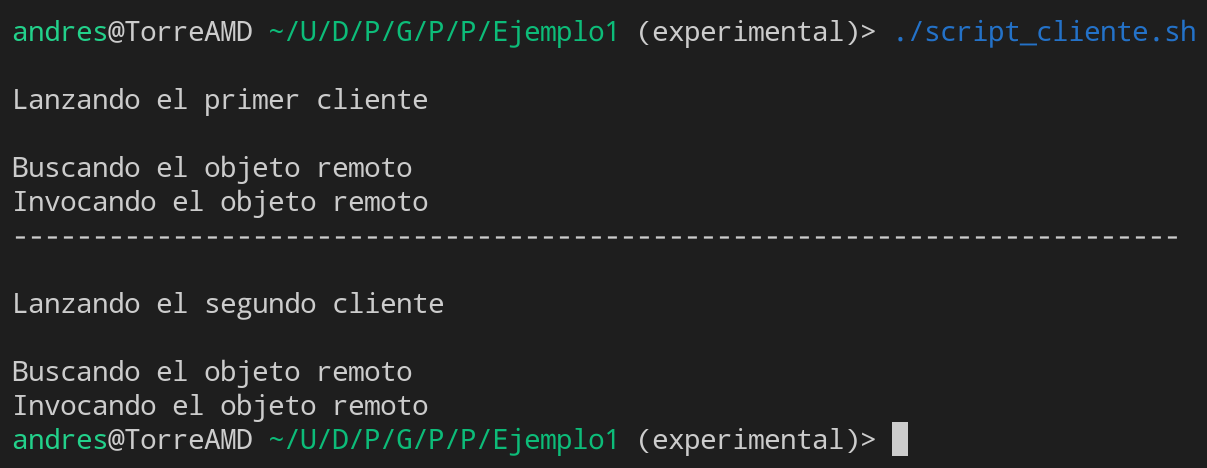
\includegraphics[width=\textwidth]{imagenes/E1C.png}
    \caption{Salida de los clientes}
\end{figure}

\subsubsection{Implementación}
Para la implementación de este sistema primero es necesario realizar la interfaz remota del servidor que va a exportar los métodos a los clientes. En este caso solo se exporta el método \textit{escribir\_mensaje}.

En la parte del servidor se crea una clase que implementa los métodos de la interfaz remota ``Ejemplo\_I''.

El método imprime por la pantalla del servidor (remota) que ha recibido la petición del proceso. Además comprueba si el número de proceso es 0, en caso afirmativo se manda el cliente que ha llamado al método remoto a dormir durante 5 segundos y luego, con independencia de que sea el proceso 0 ó no, se indica el identificador del cliente en la pantalla remota.

En la parte del main del servidor activa el gestor de seguridad, que es exactamente igual para el cliente, crea una instancia de del objeto remoto y por último se exporta y se registra en ``rmiregistry'' para que los clientes puedan encontrarlo.

En la parte del cliente se activa el gestor de seguridad accede al ``rmiregistry'' que se encuentra en la dirección pasada por consola, y obtiene a partir del registro el stub del objeto remoto para poder lanzar el método anteriormente mencionado.


\subsubsection{Funcionamiento}
El diagrama del sistema (sin incluir rmiregistry ni stubs, solo los propios objetos y clases) es el siguiente:

\begin{figure}[H]
    \centering
    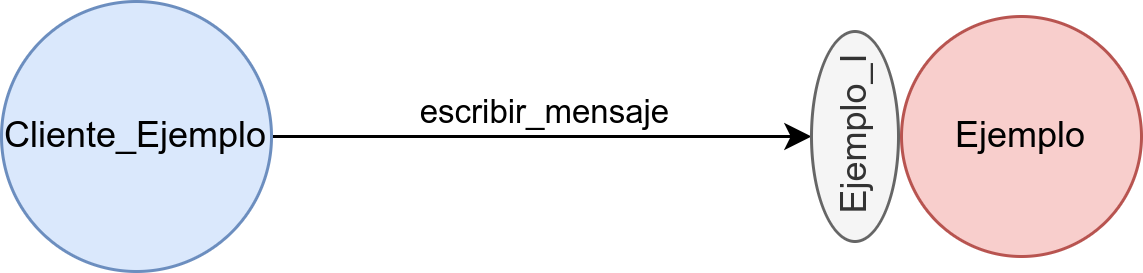
\includegraphics[width=0.5\textwidth]{imagenes/E1Diagrama.png}
    \caption{Diagrama con las comunicaciones que se realizan}
\end{figure}

Se puede ver que el cliente llama al método escribir\_mensaje exportado por la interfaz remota del servidor, que se llama Ejemplo.

\subsection{Ejemplo 2}
\subsubsection{Descripción}
En este ejemplo se realiza algo similar al anterior, pero esta vez el cliente lanza un número de hebras que se pasan por consola. La lógica del servidor es exactamente igual al ejemplo anterior (y la del cliente también, pero es con hebras).

\textbf{¿Se entrelazan los mensajes?: }Sí existe entrelazamiento. Tras varias ejecuciones se puede observar como se produce un entrelazamiento de mensajes de salida en el servidor en el que se muestra que entran varias hebras a la vez antes de que la primera haya mostrado el mensaje de salida y luego cuando salen muestra varias veces también el mensaje de salida. Puede que esto sea algo no deseado y que siempre se desee que las hebras siguientes esperen a que la hebra que va delante reciba la respuesta del servidor para que siempre haya como mucho una hebra en el método remoto.

\begin{figure}[H]
    \centering
    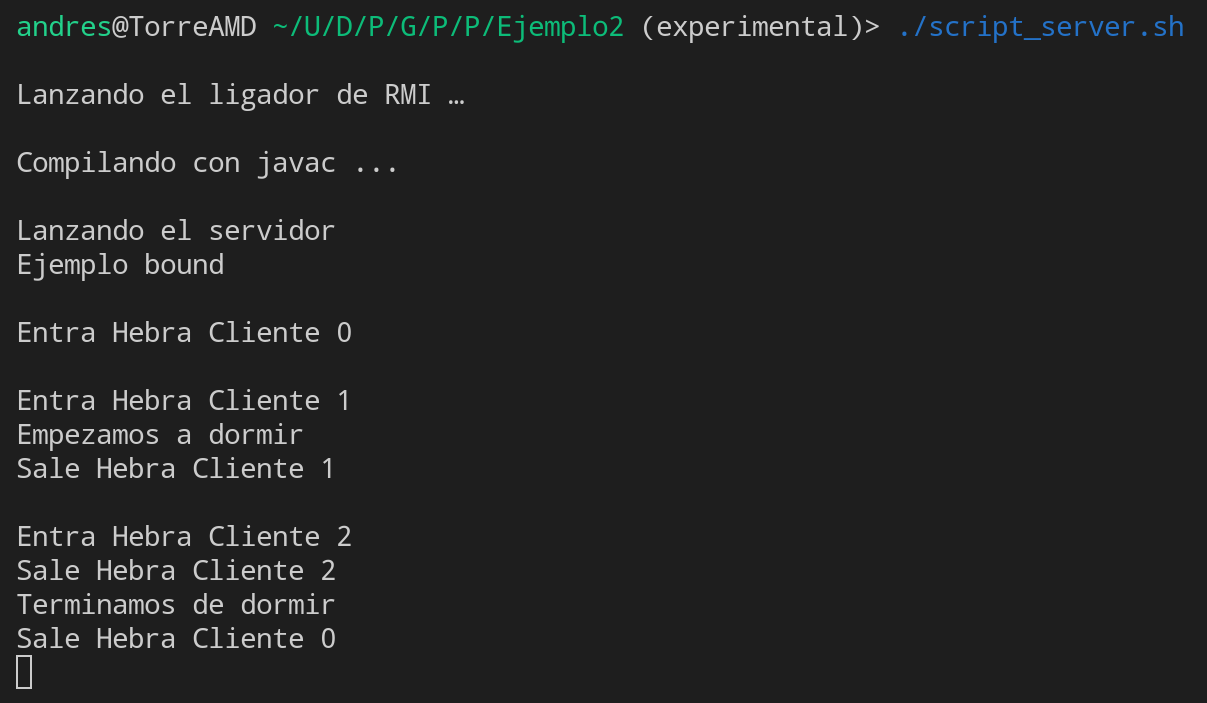
\includegraphics[width=0.7\textwidth]{imagenes/E2Server1.png}
    \caption{Entrelazamiento entre los mensajes de la hebra cliente 0 y 1}
\end{figure}

\begin{figure}[H]
    \centering
    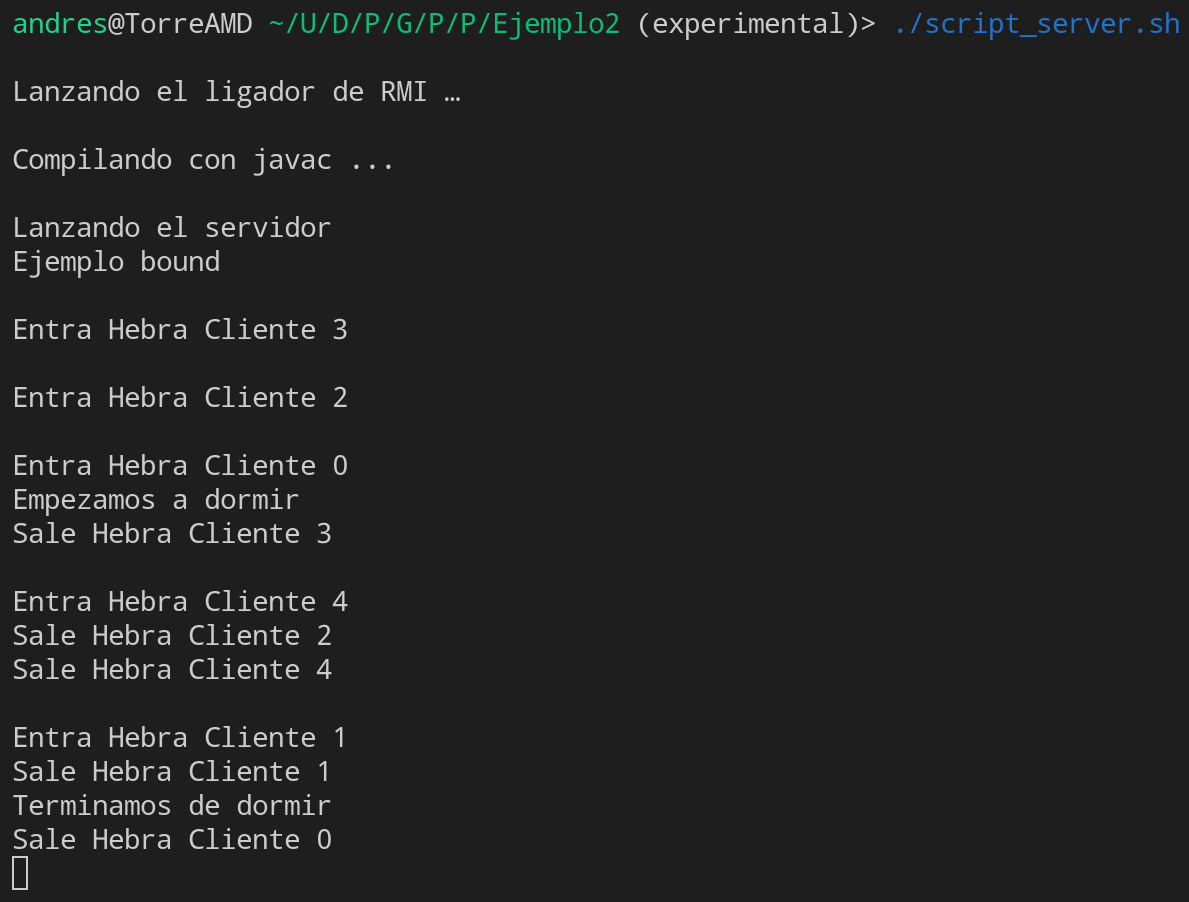
\includegraphics[width=0.7\textwidth]{imagenes/E2Server2.png}
    \caption{Entrelazamiento entre los mensajes de las hebras 0, 2, 3 y 4.}
\end{figure}

Otro entrelazamiento menor que ocurre es que las hebras no realizan las peticiones de manera ordenada al servidor; es decir, en la impresión que realiza el servidor por consola se puede observar que no siguen un orden ascendente los identificadores de los clientes. Puede ser porque realmente las hebras del cliente no llamen al método remoto en el mismo orden en que se crean (las hebras). Esto se puede ver en la imagen anterior.

\bigskip

\textbf{¿Qué hacen las demás hebras?: }Las demás hebras no esperan a que la hebra de delante reciba la respuesta del método remoto haciendo que el servidor esté ejecutando el mismo método concurrentemente produciendo así, como se ha dicho anteriormente, entrelazamientos.  
Esto implica que si el método tuviera una sección crítica, por ejemplo una escritura a una variable, se podría producir en algún entrelazamiento una condición de carrera invalidando el valor de la variable, que debería haber sido atómica. Es por eso que es necesario aplicar técnicas de sincronización (cerrojos, semáforos, monitores, etc.) entre clientes/hebras para un correcto estado del objeto que exporta el servidor.

%MOSTRAR TAMBIEN UNA FOTO SOBRE ESO
%MOSTRAR UN DIAGRAMA CON LOS POSIBLES ENTRELAZAMIENTOS, POR EJEMPLO HACER PARA EL CASO DE 3 HEBRAS
Por ejemplo, para el caso de 2 hebras se podrían dar los siguientes entrelazamientos de mensajes (supongo que son la hebra 1 y 2 para evitar entrelazamientos especiales con el bloqueo de la hebra 0):

\begin{center}
    \centerline{
        \begin{tabular}{ | c | c | c | c | c | c | }
            \hline
            Entra Hebra 1 & Entra Hebra 1 & Entra Hebra 1 & Entra Hebra 2 & Entra Hebra 2 & Entra Hebra 2 \\
            Sale Hebra 1 & Entra Hebra 2 & Entra Hebra 2 & Entra Hebra 1 & Entra Hebra 1 & Sale Hebra 2 \\
            Entra Hebra 2 & Sale Hebra 1 & Sale Hebra 2 & Sale Hebra 2 & Sale Hebra 1 & Entra Hebra 1 \\
            Sale Hebra 2 & Sale Hebra 2 & Sale Hebra 1 & Sale Hebra 1 & Sale Hebra 2 & Sale Hebra 1 \\
            \hline
        \end{tabular}
    }
\end{center}

\textbf{¿Qué ocurre con las hebras cuyo nombre acaba en 0?: }Las hebras que acaban en 0, al igual que en el ejemplo 1, se ponen a dormir durante 5000 ms (5 segundos) al llamar al método remoto. Durante ese tiempo, otras hebras pueden invocar al método remoto para su ejecución y este se ejecuta paralelamente a los otros, como se ha mencionado anteriormente. Esto hace que pueda haber instancias en el servidor que estén durmiendo e instancias que se estén ejecutando concurrentemente.

\subsubsection{Implementación}
La implementación de la parte del servidor es exactamente igual que en el ejemplo 1, salvo por algún ligero cambio del mensaje que se muestra por pantalla.


%ESTA ULTIMA PARTE ES NECESARIA COMPROBARLA
En la parte del cliente se realiza prácticamente lo mismo, pero se encapsula en el método \textit{run}, ya que son hebras, luego desde el main se crea un array de hebras y se lanzan con \textit{start}.

\subsubsection{Uso de \textit{synchronized}}
Cuando se añade la palabra clave \textit{synchronized} al método remoto del servidor ya no se produce entrelazamientos. Sin embargo las hebras que acaban en 0 se ponen a dormir y bloquea al servidor para recibir más peticiones al mismo método produciendo así posibles esperas innecesarias. Según la documentación, cuando más de una hebra llama a métodos que tienen \textit{synchronized}, solo entra uno de ellos y los demás se quedan bloqueados esperando a que salga el de delante. Esto implica que el bloqueo no solo se puede dar en una llamada a un método en concreto, sino también en varios métodos con esta palabra clave.

\begin{figure}[H]
    \centering
    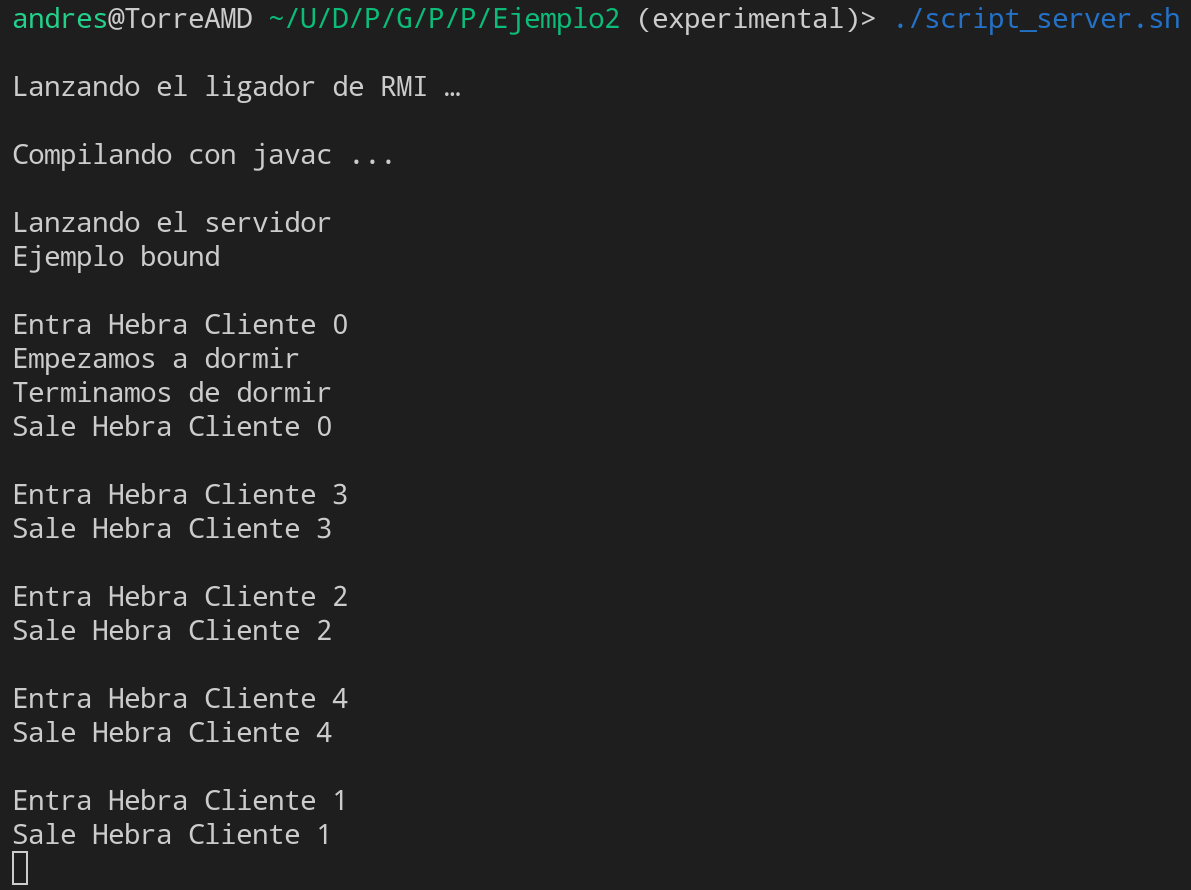
\includegraphics[width=0.7\textwidth]{imagenes/E2ServerSync1.png}
    \caption{Salida por pantalla del servidor.}
\end{figure}

Como se puede observar, la hebra 0 empieza a dormir y las demás hebras no pueden ejecutar el método hasta que se cumpla el periodo de dormir. Esto arreglaría el entrelazamiento, pero a costa de introducir esperas innecesarias, ya que ahora el método se comporta como si fuera monohebrado.

Como conclusión se puede decir que la principal diferencia entre no usar \textit{synchronized} y sí usarlo es que en el primero las hebras no necesitan esperar a que salgan las de delante para que su petición pueda ser procesada. Mientras que en el segundo caso solo una hebra puede acceder a métodos \textit{synchronized} y las demás tienen que esperar su finalización para que puedan acceder.

\begin{figure}[H]
    \centering
    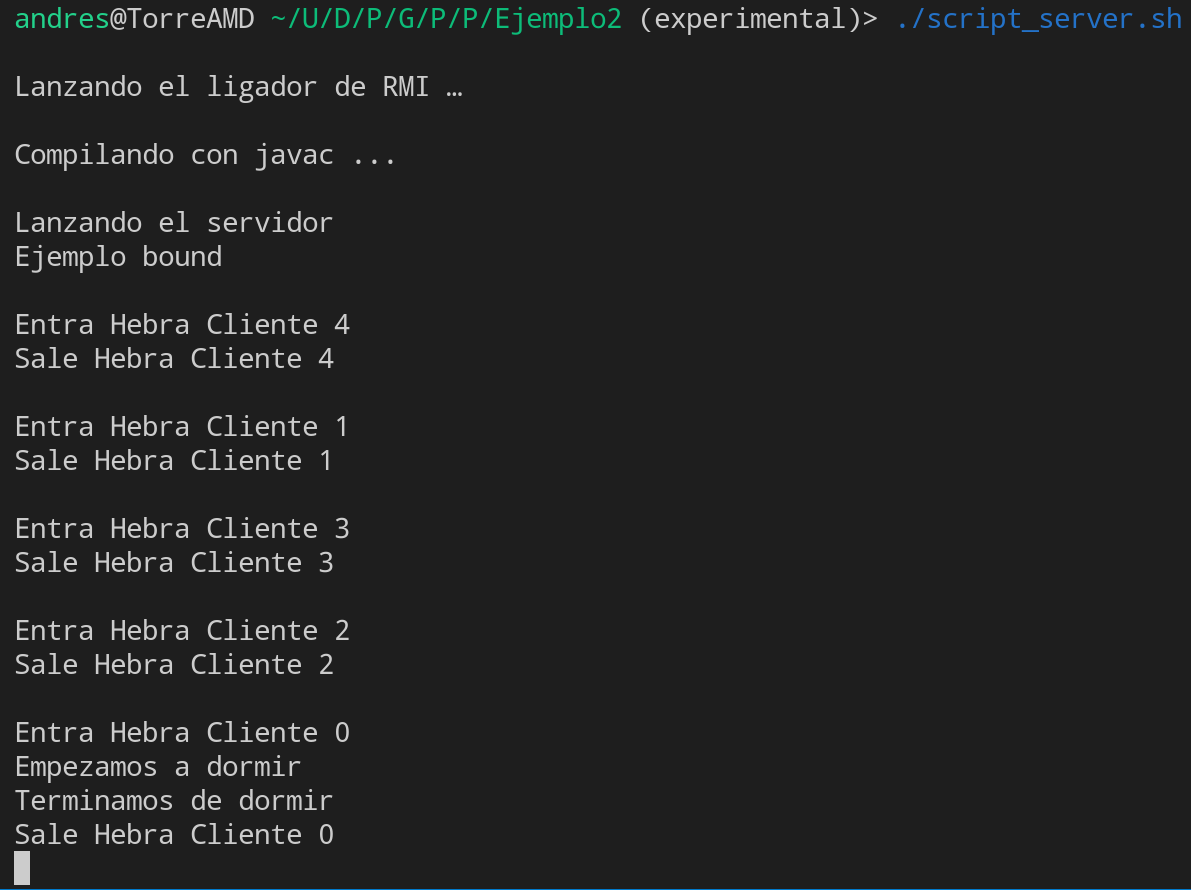
\includegraphics[width=0.7\textwidth]{imagenes/E2ServerSync2.png}
    \caption{Otra salida por pantalla del servidor.}
\end{figure}

Por último, el diagrama de la relación entre objetos es el siguiente (como antes, obviando stubs y rmiregistry):

\begin{figure}[H]
    \centering
    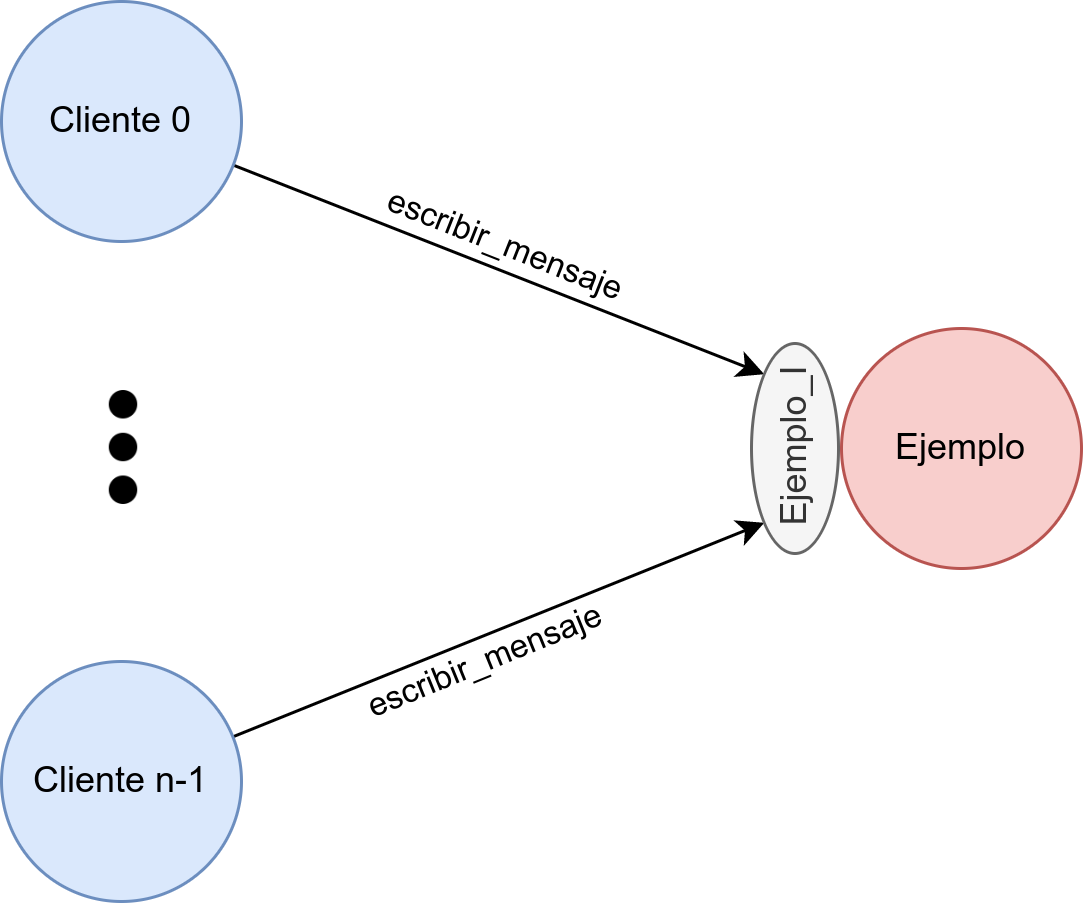
\includegraphics[width=0.5\textwidth]{imagenes/E2Diagrama.png}
\end{figure}

\subsection{Ejemplo 3}
\subsubsection{Descripción}
En este ejemplo se separa el propio objeto remoto del servidor. Para ello se crea la interfaz remota como en los ejemplos anteriores, pero esta vez se implementa en una clase aparte sin tener un main asociado.

El main se encuentra en otra clase servidor que se encarga como en los demás ejemplos de crear la instancia del objeto remoto y exportarlo al \textit{rmiregistry}.

\bigskip

Por la parte del cliente realiza la misma tarea que en los ejemplos anteriores, pero esta vez una vez creado el stub pone el contador a 0, ya que es posible que otros procesos hayan modificado el atributo ``suma''. Una vez realizado esto toma el tiempo de entrada y realiza 1000 llamadas al método remoto \textit{incrementar}, cuando acaba de realizar las llamadas toma el tiempo de salida y muestra por consola el tiempo que ha tardado y, haciendo una llamada al método getter remoto \textit{sumar}, obtiene el valor del atributo del objeto remoto, que en caso de no haber sido accedido por otros procesos o hebras será el mismo número que el de llamadas RMI realizadas, que es 1000.

%MOSTRAR IMAGEN DE ESTO Y QUIZAS AÑADIR ALGO MAS

\begin{figure}[H]
    \centering
    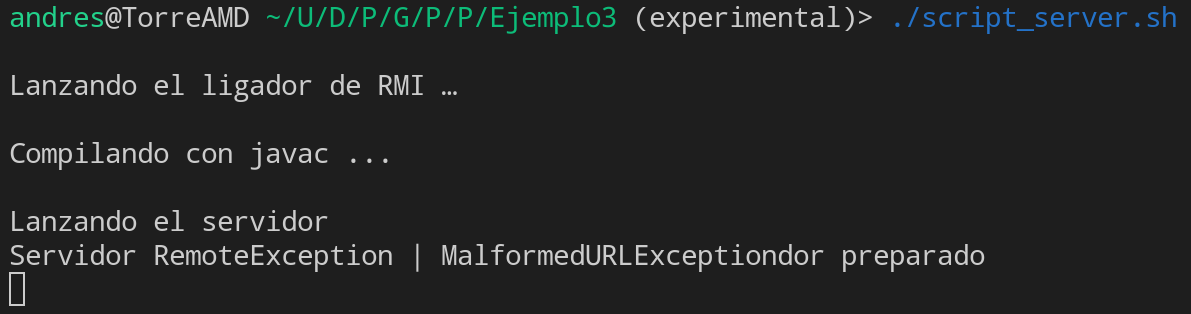
\includegraphics[width=0.7\textwidth]{imagenes/E3S1.png}
    \caption{Salida por pantalla del servidor}
\end{figure}

\begin{figure}[H]
    \centering
    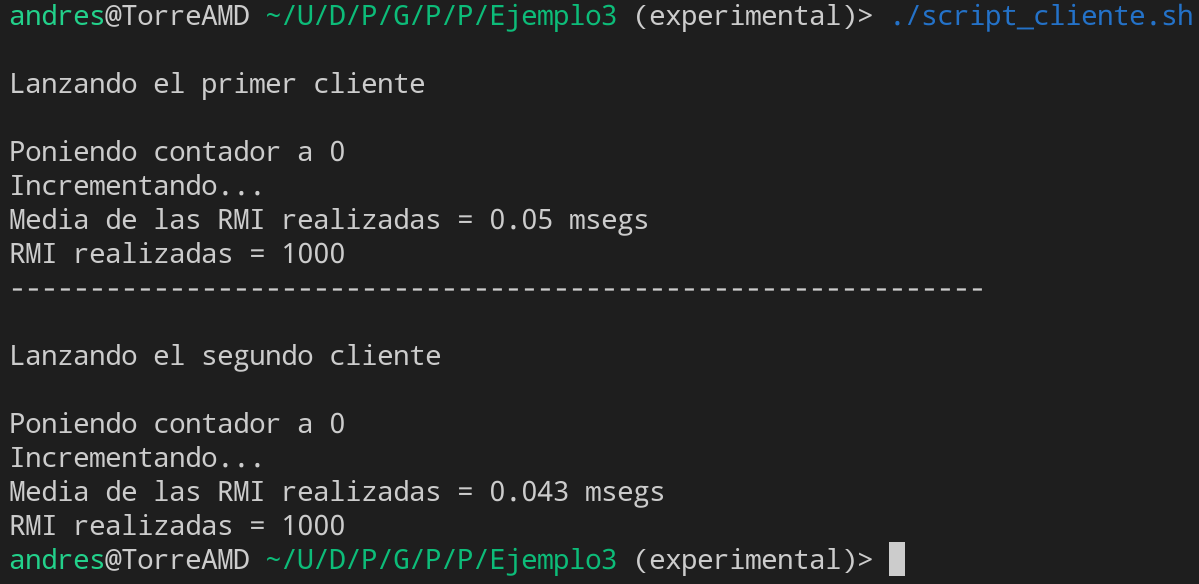
\includegraphics[width=0.7\textwidth]{imagenes/E3C1.png}
    \caption{Salida por pantalla de los clientes (delimitados por ``-'')}
\end{figure}

Por último, como en los ejemplos anteriores, un diagrama con las relaciones entre objetos:

\begin{figure}[H]
    \centering
    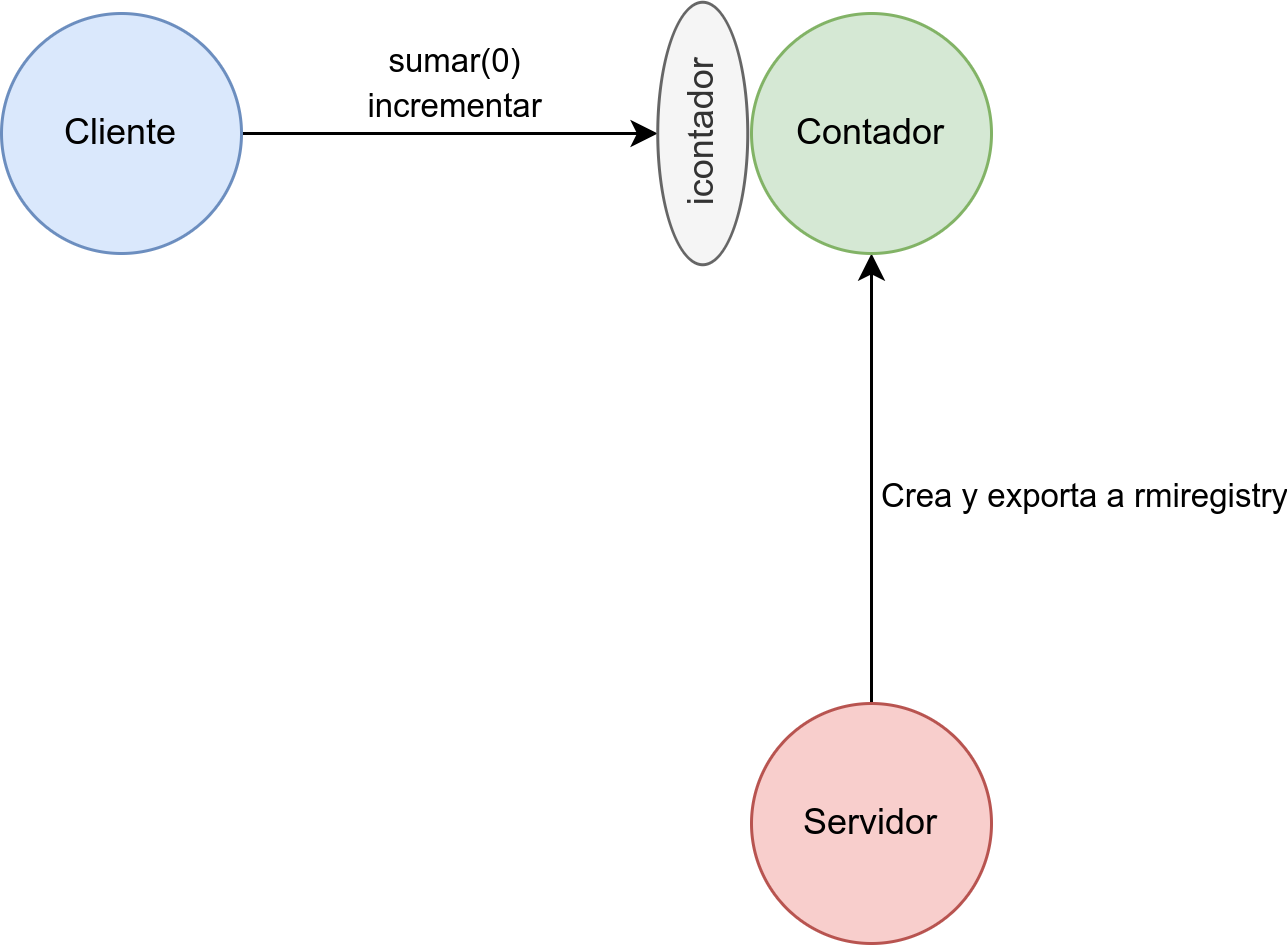
\includegraphics[width=0.5\textwidth]{imagenes/E3Diagrama.png}
\end{figure}

\subsection{Diferencias entre los ejemplos}
En estos 3 ejemplos se han visto varios aspectos importantes de RMI que hace que los diferencien en cierta medida. 

La primera diferencia es que en los ejemplos 1 y 3 se usan solamente los procesos como tal en los que no existen hebras, sino los propios procesos (JVM). Mientras que en el ejemplo 2 el cliente lanza varias hebras que acceden concurrentemente a un método remoto.

La segunda diferencia es en la implementacion de la interfaz remota, en la que en los ejemplos 1 y 2 se realiza en la propia clase del servidor mientras que en el ejemplo 3 se realiza en una clase aparte, haciendo que el servidor solo se encargue de crear la instancia remota y exportarla. Esto permite separar la implementación del objeto remoto del propio código del servidor.

Otra diferencia se encuentra en el uso de \textit{rmiregistry}, el servidor en los ejemplos 1 y 2 supone que se ha lanzado el rmiregistry y solo se encarga en exportar el objeto remoto, mientras que en el ejemplo 3 es el propio servidor el que crea el rmiregistry y le asigna un puerto mediante el método \textit{createRegistry}, es más, si se intenta lanzar rmiregistry primero y luego este servidor va a dar error por lo que es necesario matar a todos los procesos que el sistema tenga.

%MOSTRAR EL ERROR EXPLICADO EN EL PARRAFO ANTERIOR
\begin{figure}[H]
    \centering
    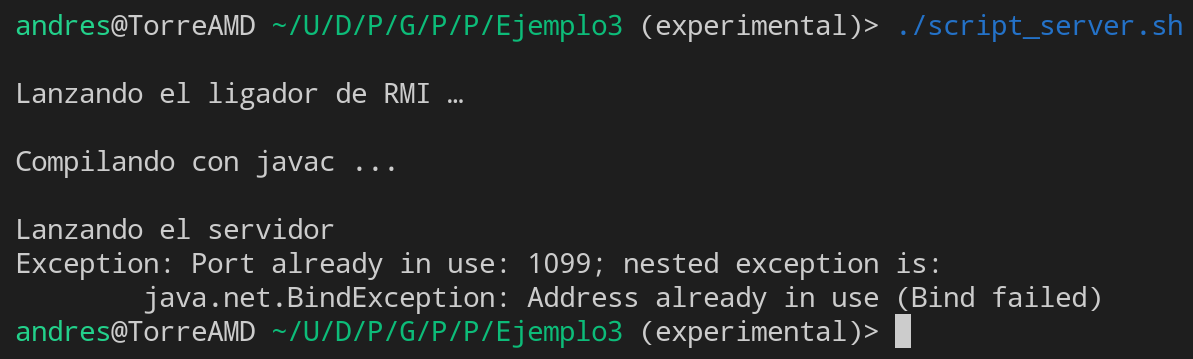
\includegraphics[width=0.7\textwidth]{imagenes/E3Error.png}
    \caption{Error al lanzar el servidor si ya se está ejecutando rmiregistry previamente.}
\end{figure}


\section{Segunda parte, servidor de donaciones}
\subsection{Descripción}
En esta parte de la práctica se pide realizar un servidor de donaciones replicado y balanceado al que los clientes se conectarán para realizar donaciones. Cuando un cliente nuevo se registre en cualquiera de las réplicas, este le registrará en la réplica correspondiente que tenga menos usuarios suscritos.

Adicionalmente, se pueden añadir métodos nuevos con funcionalidad distinta o arreglar el problema de la exclusión mutua con alguno de los algoritmos vistos en clase de teoría.

En mi caso he implementado el algoritmo de exclusión mutua en anillo para solucionar diversos problemas de entrelazamiento entre distintas réplicas y el uso de la palabra clave \textit{synchronized} para el acceso concurrente entre clientes de una misma réplica que se comentarán más abajo. También he añadido dos métodos nuevos al servidor.
\subsection{Implementación}
\subsubsection{Parte obligatoria}

Para implementarlo he decidido realizar dos interfaces remotas para el servidor de donaciones: una primera denominada ``IDonacionesInterno'' que servirá para la interconexión entre réplicas y otra llamada ``IDonacionesExterno'' que usarán los clientes para comunicarse con estas réplicas.

%MOSTRAR DIAGRAMA DE LAS REPLICAS CON LAS INTERFACES

La clase ``Servidor'' (la réplica) implementa estas dos interfaces más algunos métodos internos que no son necesarios ser exportados por ninguna interfaz.


Esta clase consta de los siguientes atributos:
\begin{itemize}
    \item \textbf{numReplicas: }Atributo de instancia que contiene el número de réplicas que se han instanciado. Principalmente sirve para realizar cálculos con bucles sobre estas réplicas.
    
    %IMPORTANTE LINKAR A LA EXPLICACION MAS ABAJO
    %IMPORTANTE EXPLICAR TRANSACCIONES CLIENTES
    \item \textbf{datosClientes: }Map de entero y \textbf{TransaccionesClientes} (explicación en la sección de la parte extra) donde se almacenan para cada cliente el historial de donaciones junto con la fecha en la que se ha realizado (todo esto dentro de TransaccionesClientes).
    \item \textbf{credencialesClientes: }Otro Map en el que se almacena para cada cliente su contraseña. Esto se usa para darle más realismo a la práctica dando la sensación de existir un login.
    \item \textbf{idServer: }Contiene el identificador de la réplica.
    \item \textbf{subTotal: }Contiene el subtotal donado por los clientes en esa réplica. Este atributo luego se usa para obtener el total global donado. 
    \item \textbf{direccion: }Contiene la dirección que se va a utilizar, por defecto es ``localhost''.
\end{itemize}

%Mostrar ejemplo de ejecucion para mas de dos replicas


El main del servidor crea un número de réplicas que se pasan por consola y las exporta a ``rmiregistry'' con el identificador ``S\#'' donde `\#' es el identificador de la réplica. Una vez realizado esto lo que hace es mostrar continuamente el total que tienen todas las réplicas por consola.

El funcionamiento básico cliente/réplica en el main del cliente se consigue, lo primero de todo, registrando al cliente en el sistema, se le asigna una réplica y a partir de ese momento es capaz de realizar diversos métodos que se explicarán más abajo.

Además, una vez registrado en el sistema, se puede volver a iniciar sesión proporcionando el identificador del cliente y la contraseña como si de unos credenciales se tratasen y, en caso de ser incorrectos, no se puede realizar ninguna operación.

A continuación se muestran los métodos que pueden usar los clientes (los básicos, en la siguiente sección explicaré los demás).

\begin{itemize}
    \item \textbf{registrarCliente: }Se encarga de registrar a un cliente en la réplica con menor número de clientes suscritos y devuelve el identificador de la réplica en la que se ha registrado. Además también hace las veces de método para iniciar sesión, ya que si se llama con los credenciales de un cliente ya registrado, devuelve el identificador en el que se encuentra. También si se pasa un identificador existente, pero con una contraseña inválida, devolverá la cadena vacía para que no se pueda conectar.
    
    \item \textbf{donar: }Hace que un cliente registrado pueda donar la cantidad pasada como parámetro. En caso de no estar registrado o tener credenciales inválidos no se realiza ninguna acción y se muestra por la pantalla del servidor un mensaje informativo.

    \item \textbf{totalDonado: }Permite que un cliente registrado y que haya realizado al menos una donación obtenga el total que hay en todas las réplicas. En caso de no estar registrado, tener unos credenciales inválidos o no haber donado se devuelve el valor -1.
    
    \item \textbf{totalDonadoCliente: }Obtiene el total que ha donado un cliente. Realiza las comprobaciones que los métodos anteriores y si fallan se devuelve -1.\
    
    \item \textbf{getNombreReplica: }Obtiene el nombre de la réplica tal y como se exporta en rmiregistry.
\end{itemize}

Mientras que para la intercomunicación entre réplicas (como antes, sólo lo obligatorio, en la siguiente sección explicaré los métodos del algoritmo de exclusión mutua):

\begin{itemize}
    \item \textbf{clientesSize: }Obtiene el número de clientes conectados a la réplica que lo llama.
    \item \textbf{existeCliente: }Comprueba si está registrado el cliente en la réplica en la que se llama.
    \item \textbf{añadirCliente: }Añade un cliente a la réplica que llama este método. Este método no realiza comprobaciones de ningún tipo ya que se supone que se hacen en los métodos correspondientes.
    \item \textbf{getNombreReplica: }Realiza lo mismo que el método de la interfaz de los clientes.
    \item \textbf{getSubTotal: }Obtiene el subtotal de la réplica que lo llama.
\end{itemize}

\subsubsection{Parte extra}
Como extra he implementado algunos métodos que añaden funcionalidad al sistema, he arreglado el problema de la exclusión mutua de ciertos atributos y también he añadido un rol más al sistema, el administrador. Los métodos que he añadido, accesibles para los clientes, son los siguientes:


%AÑADIR EL METODO QUE FALTA
\begin{itemize}
    \item \textbf{registrarClienteInseguro: }Realiza la misma funcionalidad que el método ``registrarCliente'', pero se le quita la parte del algoritmo en anillo para la solicitud de acceso a la sección crítica. Se usa principalmente para denotar las diferencias entre ambas versiones, en el main interactivo no se usa.
    \item \textbf{ponerACero: }Permite poner a cero la cantidad total donadaen todas las réplicas además de limpiar el historial de transacciones de todos los clientes registrados. Solo los adminsitradores son capaces de retirar el dinero.
    \item \textbf{getTransacciones: }Permite obtener el histórico de donaciones (cantidad y fecha) para el cliente con los credenciales pasados por parámetro. En caso de ser incorrectos se devuelve la cadena vacía.
    \item \textbf{bloquearUsuario: }Permite bloquear a un usuario del servidor de donaciones para que no pueda realizar más acciones (nisiquiera consultar su historial de donaciones), esto incluye también no poder ver el total que hay en todas las réplicas. Sólo los administradores pueden bloquear a usuarios.
    \item \textbf{desbloquearUsuario: }Permite que un administrador desbloquee a un usuario, haciendo que este pueda realizar operaciones de nuevo con el servidor.
\end{itemize}

También, como mencioné en la sección anterior, he creado una clase ``TransaccionesClientes'' que almacena todas las operaciones que realiza un cliente, tanto la fecha y hora como la cantidad. Esto, unido con el método ``getTransacciones'' permite mostrar en el modo interactivo esta información. No es un método como tal, sino más bien una profundización de un parámetro básico que se necesitaba. Cabe recalcar que el histórico se almacena de manera independiente para todos los clientes, por lo que cada uno va a tener un historial único.

Además he añadido el rol del administrador. Los administradores tienen un identificador menor que 0 y pueden realizar acciones que los usuarios normales no pueden. Los métodos que pueden usar (que están explicados arriba) son: ``ponerACero'', ``bloquearUsuario'' y ``desbloquearUsuario''. Por razones de evitar complicar demasiado la corrección he puesto para que en el main de los clientes se puedan crear también administradores, esto en la vida real habría que limitarlo ya que cualquiera podría crearse una cuenta de administrador.

%MOSTRAR IMAGENES DE BLOQUEO DE USUARIOS TANTO POR EL ADMIN COMO MOSTRAR CUANDO ESTA BLOQUEADO QUE SALE

%MOSTRAR IMAGENES DE UN HISTORICO


%MOSTRAR FOTOS CON LOS EJEMPLOS DE EJECUCION DE LOS METODOS


Ahora bien, un problema que surge con la implementación básica es que no se puede asegurar la correcta asignación de réplicas a los clientes para que estén balanceados. Este problema puede surgir cuando, por ejemplo, dos clientes accedan concurrentemente al método ``registrarCliente'', pero en réplicas distintas, ya que puede darse el caso que en un momento dado una réplica tenga menos que las demás y se asigne esta réplica a ambos. Además, las estructuras de datos internas son modificadas y pueden darse estados inválidos.

%MOSTRAR FOTO CON EL PROBLEMA
%Asignación de clientes en dos réplicas de manera desequilibrada.

El resultado de la imagen anterior se puede reproducir ejecutando el script \textbf{CAMBIAME ES IMPORTANTE POR FAVOR HAY QUE PONER EL NOMBRE DEL SCRIPT ANTES DE ENTREGAR}

Otro problema que, si bien no se puede demostrar con un test, existe es el del acceso al total donado, ya que para calcularlo es necesario acceder a los subtotales de todas las réplicas, valor que puede cambiar mientras se realiza la operación.

También hay otro en el método ``ponerACero'' ya que tiene que modificar la variable del subtotal en todas las réplicas y la estructura de datos con el histórico de los clientes. Por tanto es necesario una sincronización ya que puede darse el caso de accesos concurrentes a este método, o un entrelazamiento con el método ``donar''.

Y uno último que he descubierto es en los métodos de administrador ``bloquearUsuario'' y ``desbloquearUsuario'', los cuales modifican estructuras de datos para llevar el recuento, por lo que es necesario una sincronización.

Una primera aproximación para garantizar la integridad entre clientes/administradores de una misma réplica es hacer los métodos ``registrarCliente'', ``ponerACero'', ``donar'', ``bloquearUsuario'' y ``desbloquearUsuario'' como \textit{synchronized}, esto hace que cuando varios clientes/administradores intenten llamar a la vez a algún método con esta palabra clave se bloqueen hasta que no salga el que está ejecutando el método.

Sin embargo esta solucion no sirve cuando hay mas de una replica ya que pueden acceder varios clientes/administradores de replicas distintas a la vez. Para ello es necesario implementar un algoritmo que garantice la exclusión mutua, en mi caso he realizado el algoritmo en anillo.

Este algoritmo consiste en un conjunto de procesos que tienen solo un token que van circulando periódicamente al siguiente realizando así un anillo. Cuando un método necesita realizar una sección crítica, solicita el token y se bloquea hasta que el proceso recibe del anterior el token, el cual bloquea la circulación del mismo al siguiente y desbloquea al cliente para que pueda ejecutar la sección crítica, asegurando así la ejecución por un único proceso. Cuando finaliza la ejecución de la sección crítica se desbloquea la ejecución de la circulación del token y sigue moviéndose hasta que otro proceso lo solicite.

Lo que he hecho ha sido crear los siguientes métodos \textbf{volátiles}:

\begin{itemize}
    \item \textbf{token: }Variable booleana que indica si el token se encuentra en la instancia de la réplica.
    \item \textbf{solicitado: }Variable que permite que un proceso solicite la entrada a una sección crítica para que posteriormente se le conceda cuando tenga el token.
\end{itemize}

Cabe destacar que las variables tienen que ser volátiles ya que si no lo son el bucle de las esperas ocupadas no funcionan. Esto es debido a que el compilador genera una optimización incorrecta:

%MOSTRAR UNA IMAGEN CON LA OPTIMIZACION INCORRECTA


También ha sido necesario implementar los siguientes métodos:

\begin{itemize}
    \item \textbf{setToken: }Método remoto que pone el valor del token de la réplica que lo llama al valor pasado por parámetro.
    \item \textbf{solicitarToken: }Pone la variable ``solicitado'' a true y espera hasta que su réplica tenga el token.
    \item \textbf{liberarToken: }Pone ``solicitado'' a false para que su réplica pueda finalmente pasar el token.
    \item \textbf{pasarToken: }Pasa el token a la siguiente réplica.
\end{itemize}

La acción de circular el token se implementa medienta hebras en las réplicas. Estas hebras lo que realizan es un bucle infinito donde se pasa el token solo si lo tiene y nadie lo ha solicitado, en otro caso no realiza ninguna instruccion mas.

El diagrama resultante sería el siguiente (obviando stubs):

\begin{figure}[H]
    \centering
    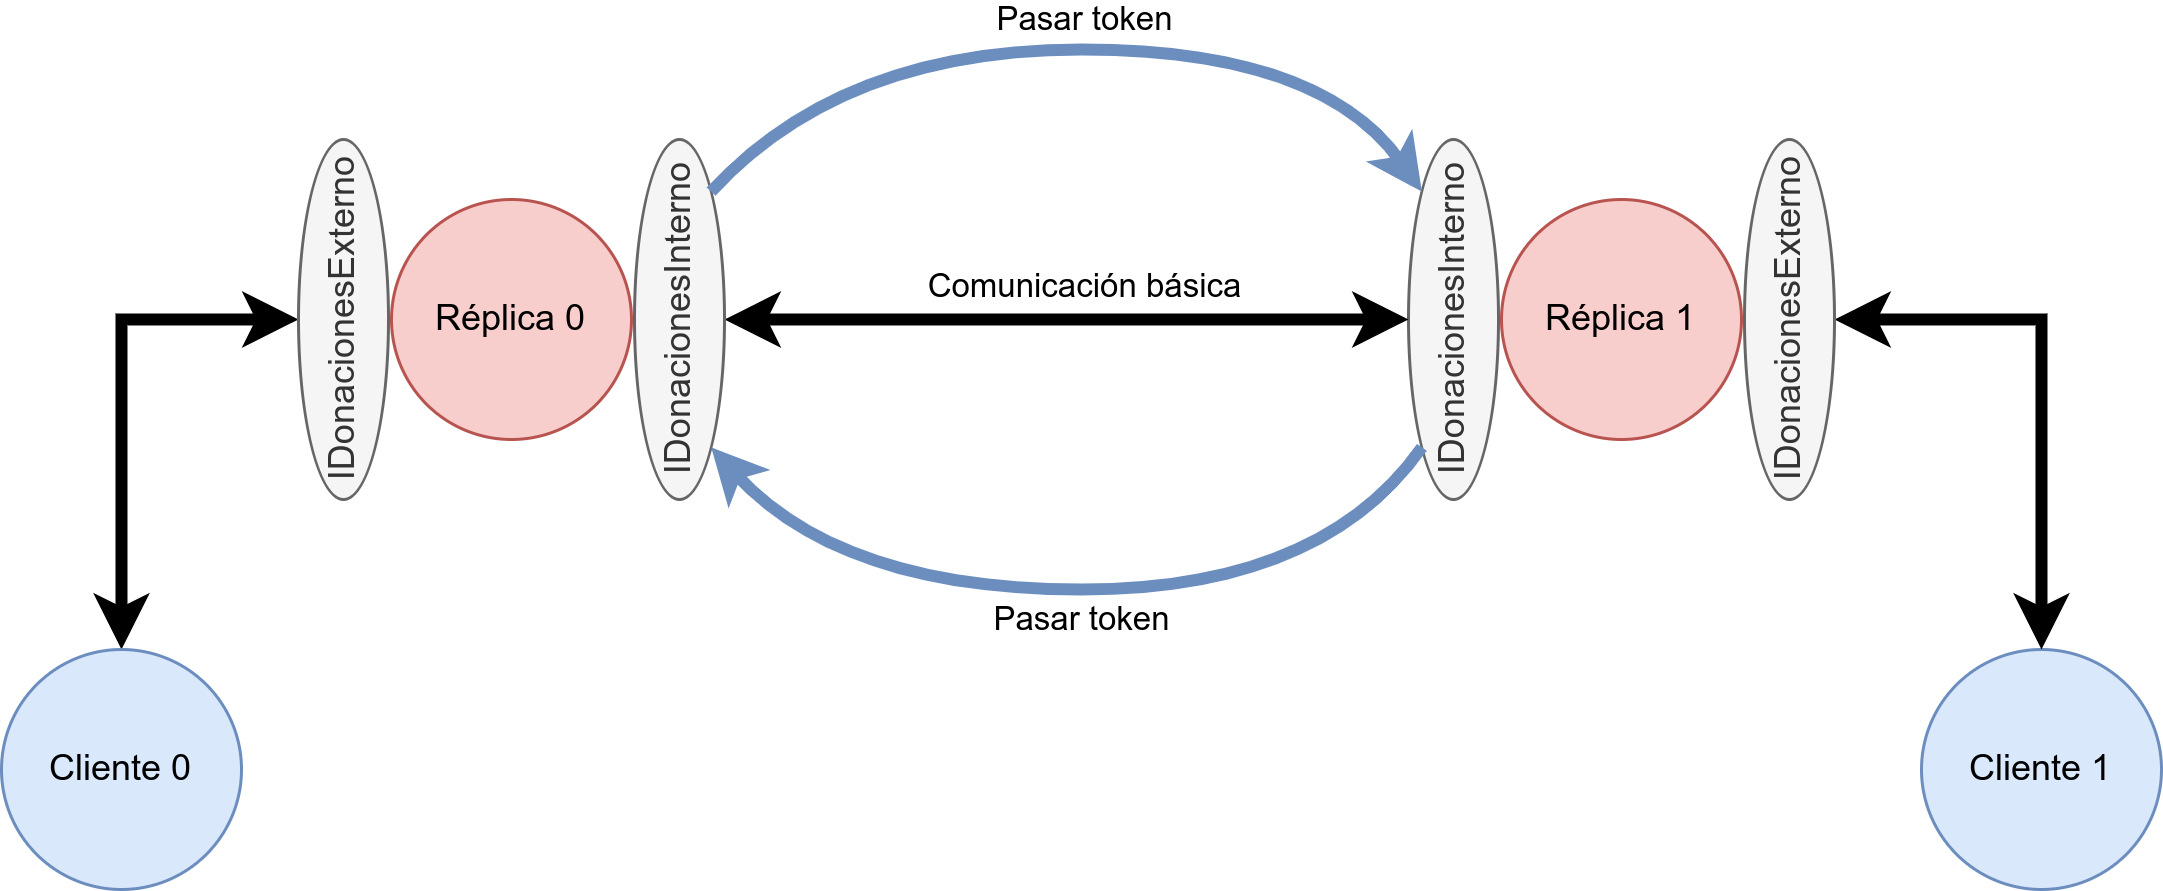
\includegraphics[width=0.7\textwidth]{imagenes/diagramaAnillo.png}
    \caption{Diagrama resultante para dos réplicas y un cliente por réplica. Las flechas negras son las comunicaciones que ya se realizaban, mientras que las azules son las del propio algoritmo.}
\end{figure}

Con esto ya sí se garantiza exclusión mutua como se puede ver en las siguientes imágenes:

%IMAGENES DE EJEMPLO DE EJECUCION QUE ANTES DABAN FALLO

\subsection{Ejecución en dos ordenadores reales}
En esta parte voy a realizar la ejecución de todo el sistema en dos ordenadores. Para ello, voy a usar dos ordenadores físicos: para las réplicas del servidor voy a usar una torre (con hostname `TorreAMD') porque es más potente, mientras que para los clientes voy a usar el portátil que me llevo a la facultad (con hostname `MSI').

Para que todo esto funcione es necesario modificar el comando de ejecución del servidor por ``-Djava.rmi.server.hostname=IP'' donde \textit{IP} tiene que ser la dirección IP donde se va a encontrar, no localhost.

Tambien es necesario cambiar el programa main del cliente para que en el metodo \textit{getRegistry} se pase la dirección IP donde se encuentra el servidor de réplicas.

RMIRegistry se va a encontrar también en TorreAMD para simplificarlo.

Por tanto, el diagrama de interconexiones seria el siguiente:

\begin{figure}[H]
    \centering
    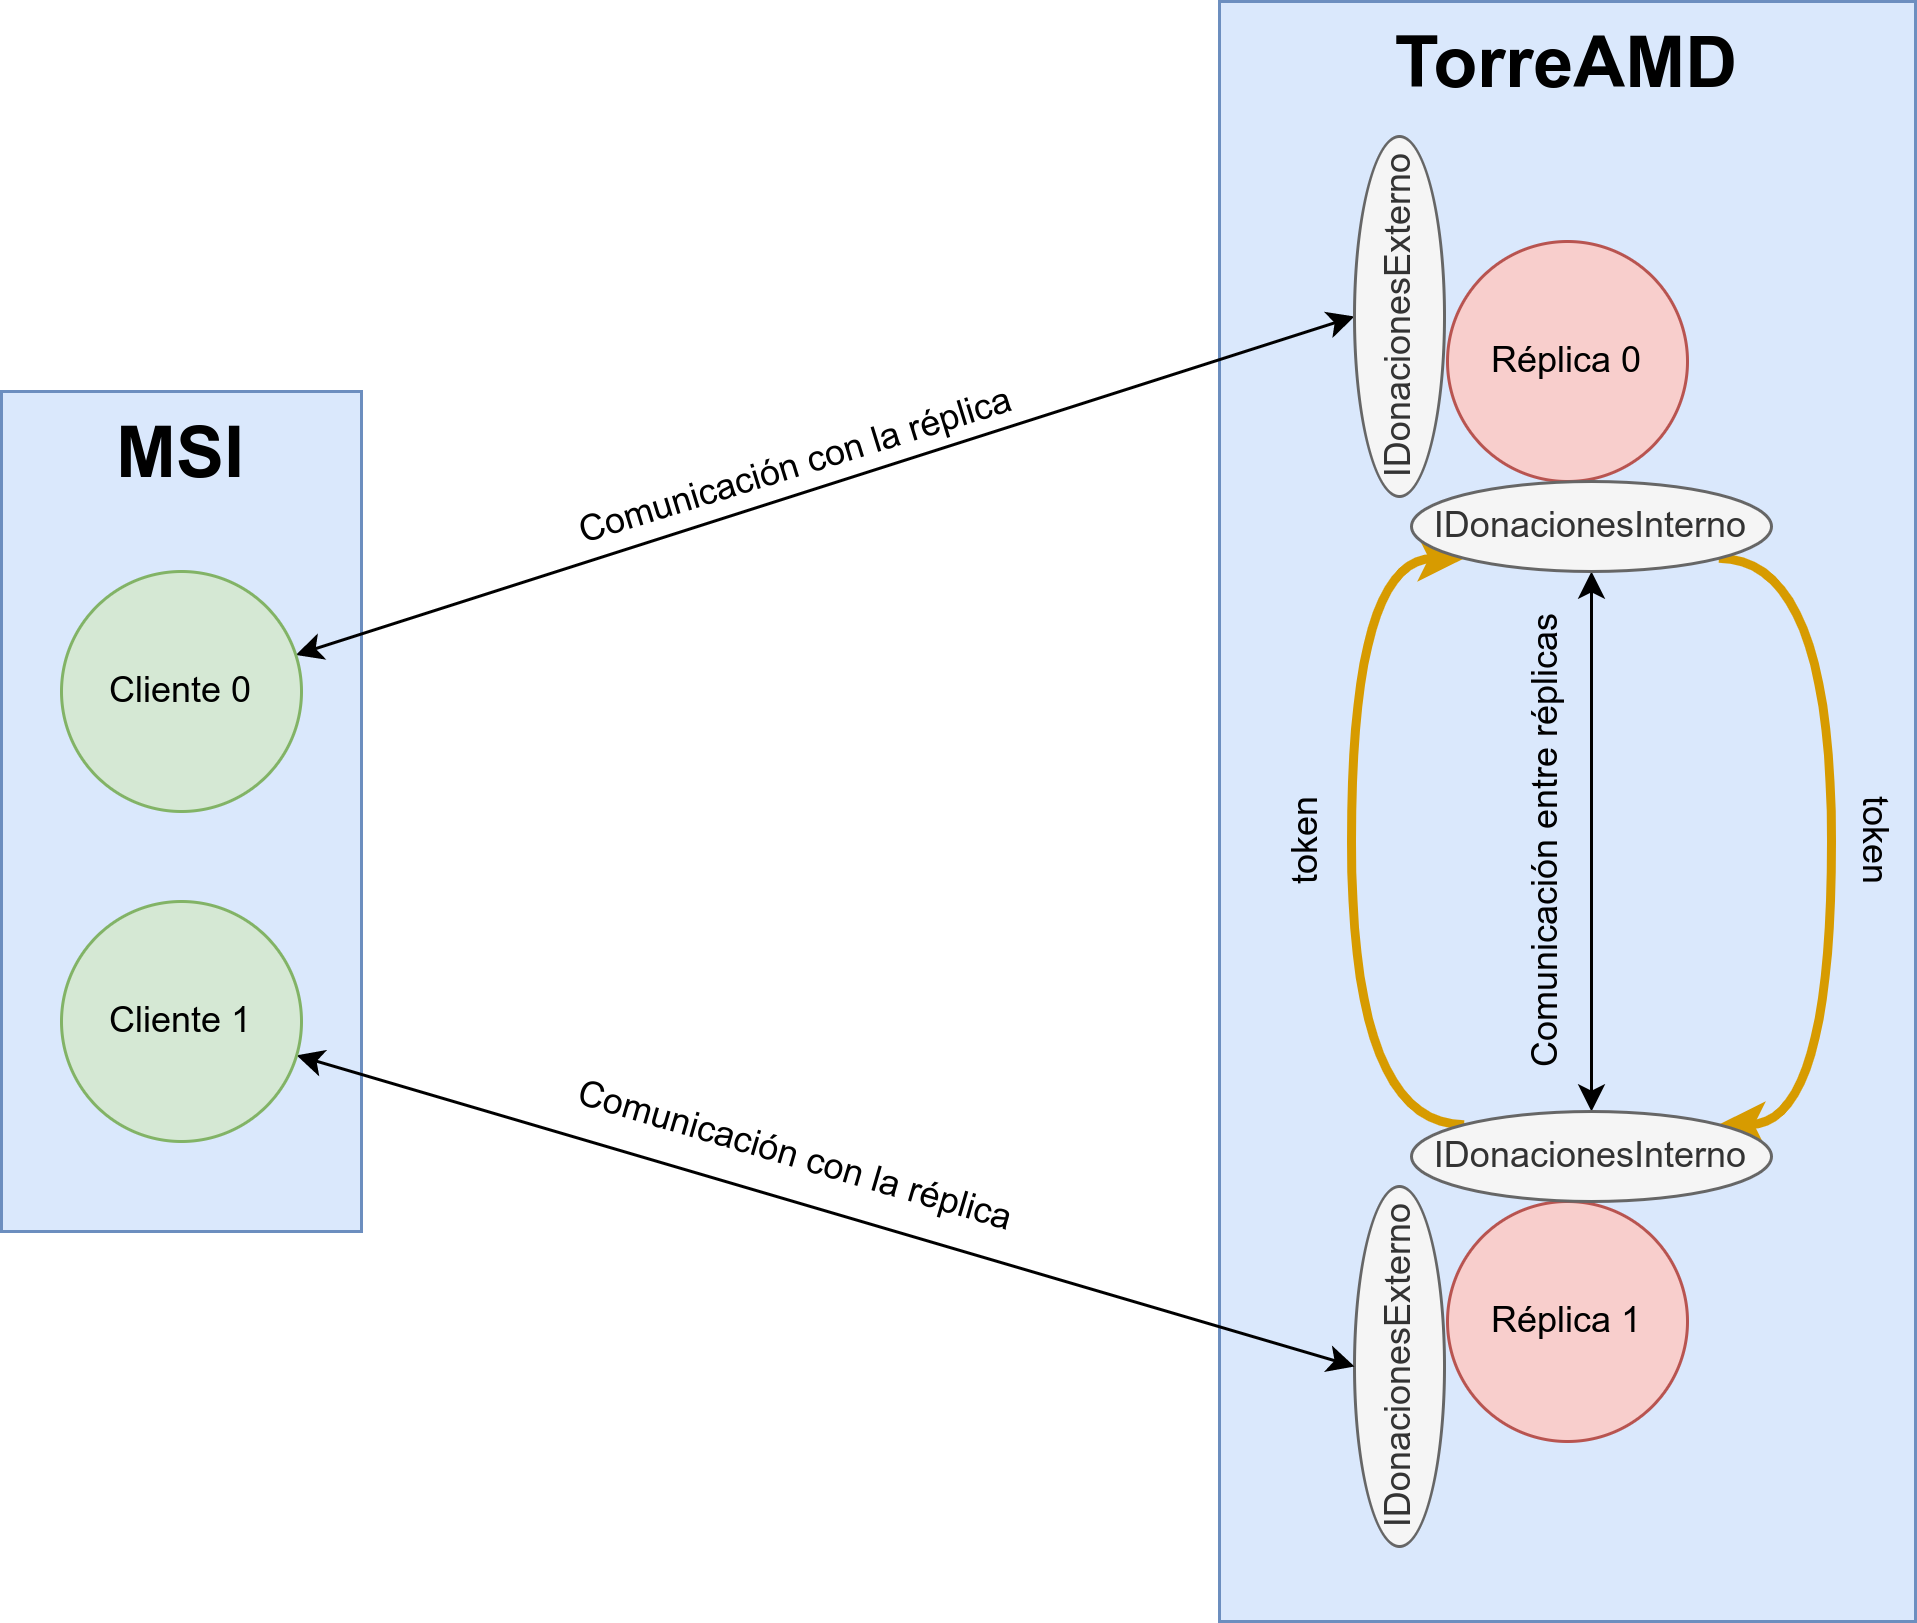
\includegraphics[width=0.7\textwidth]{imagenes/variosOrdenadores.png}
    \caption{Ejemplo de dos clientes en el portátil y dos réplicas en la torre.}
\end{figure}

Para la ejecucion en el servidor he modificado el script original para que ahora acepte como parametro, aparte del numero de replicas, la direccion IP (es de manera opcional, si no se pone el parametro se usa localhost por defecto).

Mientras que para la ejecucion en el cliente he realizado algo similar que para el servidor y he hecho que en el script se pase como parametro la direccion IP donde se encuentra el servidor (por defecto tambien a localhost).

%MOSTRAR FOTO DE IP A

Por tanto el comando de ejecucion en el servidor es el siguiente: 
%PONER EL COMANDO

MIentras que en el cliente es el siguiente: 
%PONER EL COMANDO

%MOSTRAR FOTO DE AMBOS FUNCIONANDO

Y ahora con el siguiente comando en el cliente se comprueba si sigue funcionando el algoritmo en anillo: %PONER COMANDO PARA VARIOS CLIENTES

%FOTO EN MODO INSEGURO
%FOTO EN MODO SEGURO


Como se puede ver funciona exactamente igual que todo en local, además al estar en la misma subred ambos ordenadores la latencia ha sido muy similar también.



\section{Apéndice: Implementación antigua del servidor de donaciones}
Esta sección solamente sirve para explicar mis varias implementaciones que he realizado del algoritmo en anillo hasta dar con el definitivo, que es el que se explica arriba. Esta parte solo está para una explicación, no es necesario que se tenga en cuenta.

La principal diferencia entre la versión definitiva del algoritmo y esta es que separé el propio algoritmo en una clase aparte denominada ``Anillo''. Esta clase implementaba dos interfaces remotas, una primera interna que servía para obtener atributos y modificarlos como el del token y para pasar el token de manera periódica.

\begin{figure}[H]
    \centering
    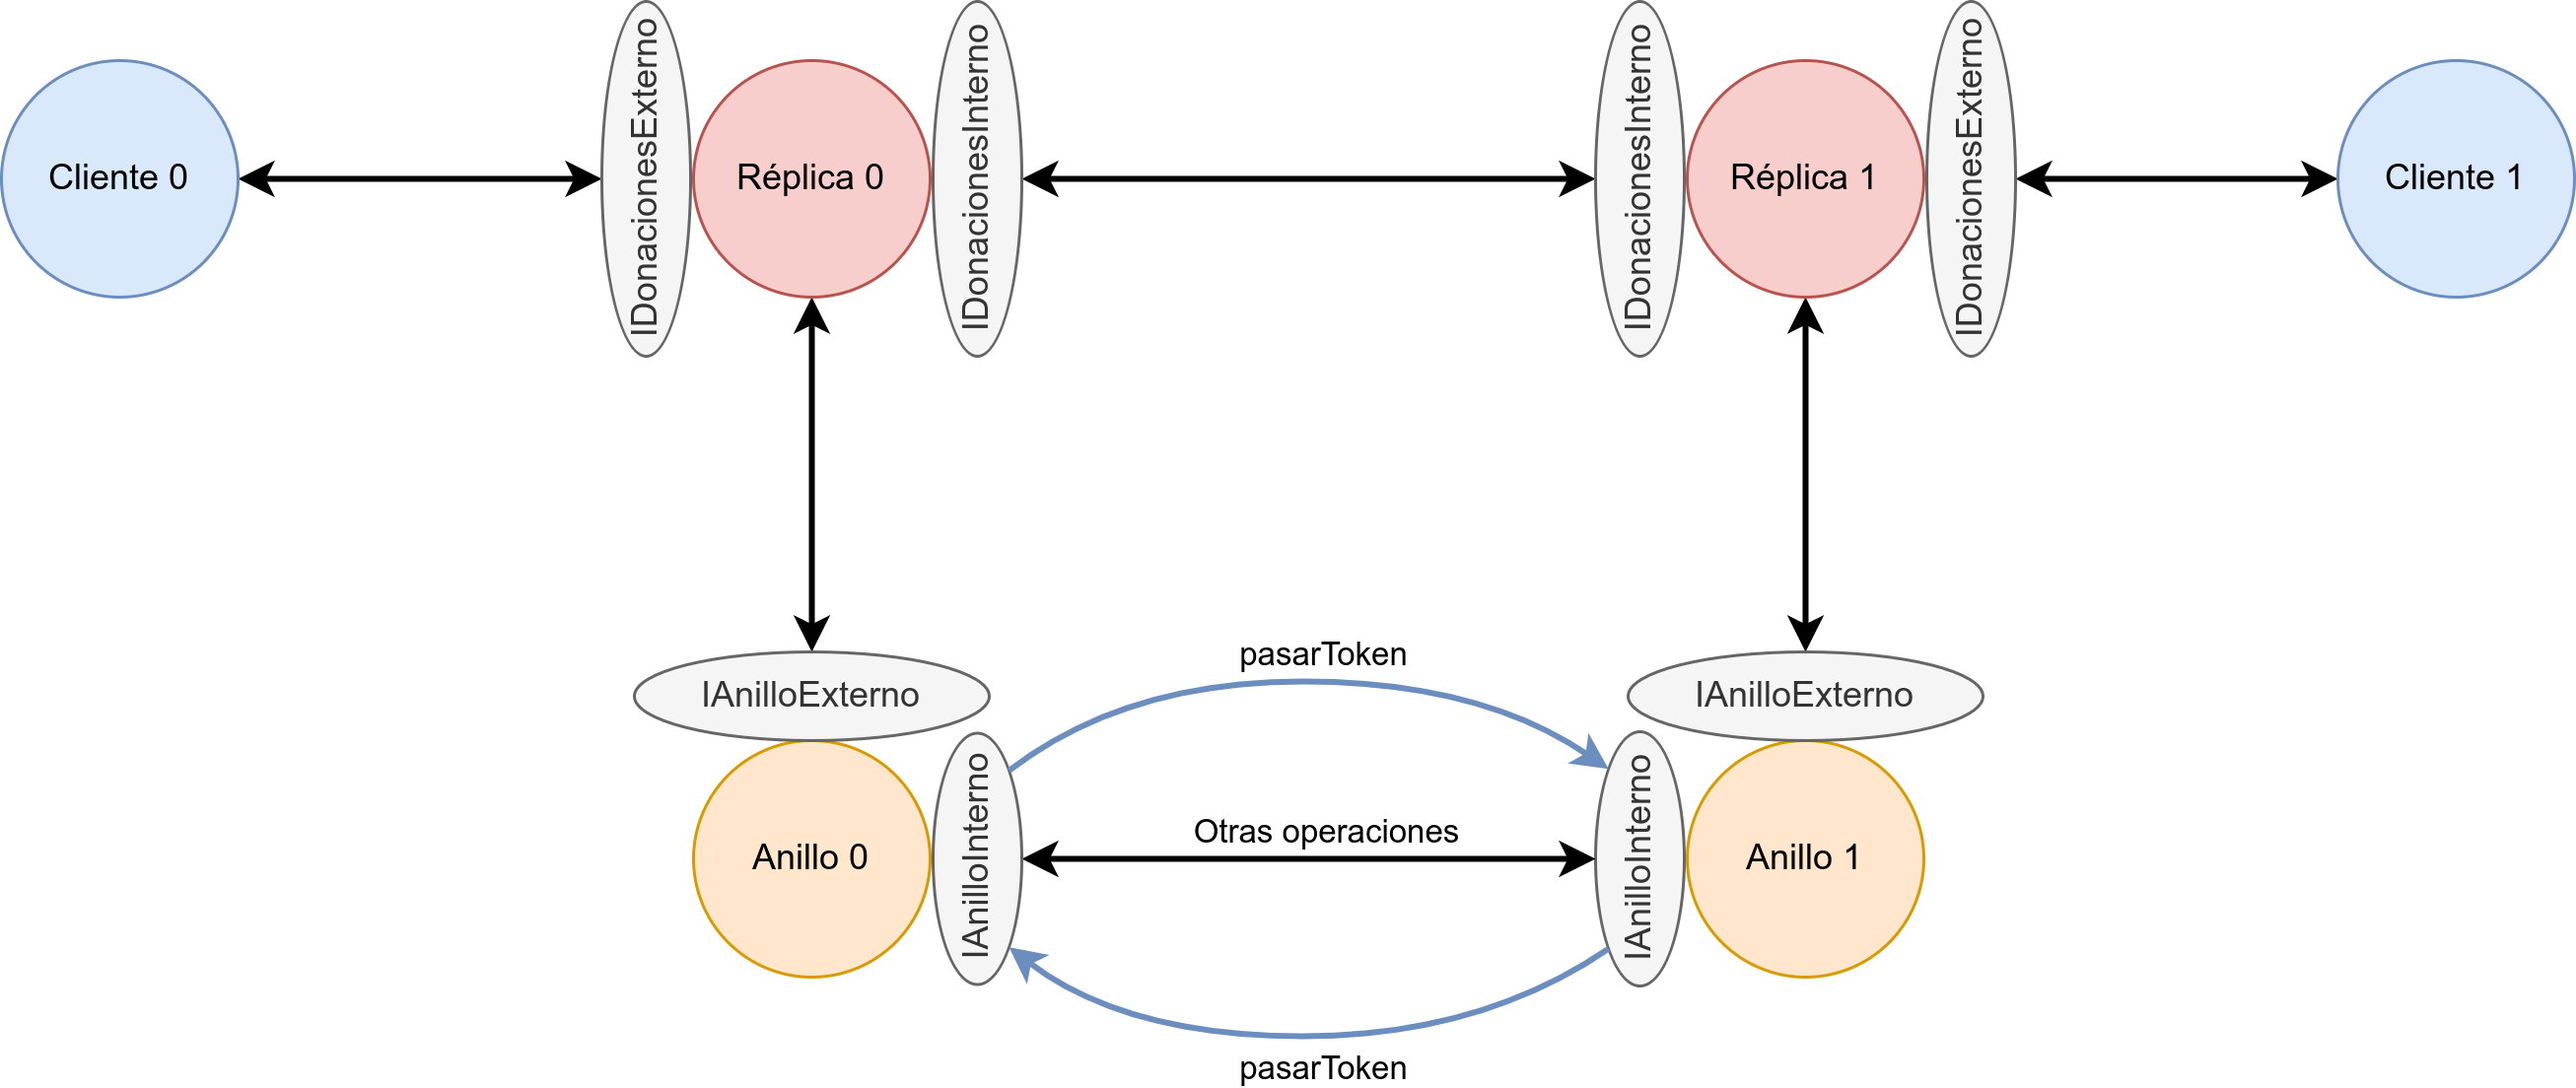
\includegraphics[width=0.7\textwidth]{imagenes/diagramaAnillosSeparados.png}
    \caption{Diagrama de interconexiones entre objetos. En azul se denota la circulación del token.}
\end{figure}

La circulación del token se realizaba desde el main del servidor, que aparte de crear y exportar las réplicas, creaba y exportaba los anillos también y a su vez con un bucle se pasaba el token al siguiente proceso.

En esta clase implementé dos versiones distintas del algoritmo: una basada en esperas ocupadas realizadas con bucles while y otra basada en esperas bloqueadas con cerrojos y condiciones de Java.

La que me convenció más al final, antes de implementar la versión definitiva fue la de espera bloqueada, ya que no se producían interbloqueos o posibles entrelazamientos incorrectos. En la versión con espera ocupada podía darse un entrelazamiento incorrecto entre el método ``solicitarToken'' y ``pasarToken''.

Estas dos implementaciones se encuentran en la carpeta ``Implementaciones antiguas'', que a su vez tiene otras dos carpetas con ambas versiones (la estructura de las prácticas se explican en la primera sección).

\end{document}